\newcommand{\thiswork}{{\color{blue}[This Work]}}
\begin{mainbox}{Background, Problem, Previous Work}
    We consider a family of one-dimensional nearest-neighbor random walks with self-interaction, called \textit{Self-interacting Random Walks} (SIRW), originally introduced and study by Toth [1].
    % : when the walker moves around the integer lattice $\mathbb{Z}$, the edges accumulate a weight that depends on the local time accumulated at the edges, and edges with higher weight tend to be visited more frequently. 
    Edges accumulate a weight that depends on the local time, according to the weight function
    \begin{equation*}
        w(n) = n^{\alpha}(1 + 2^p B n^{-p} + O(n ^{-1 - \kappa}))^{-1}, \qquad
        \alpha \in \mathbb{R}, p > 0, \kappa > 0.
    \end{equation*}

    \begin{multicols}{2}
    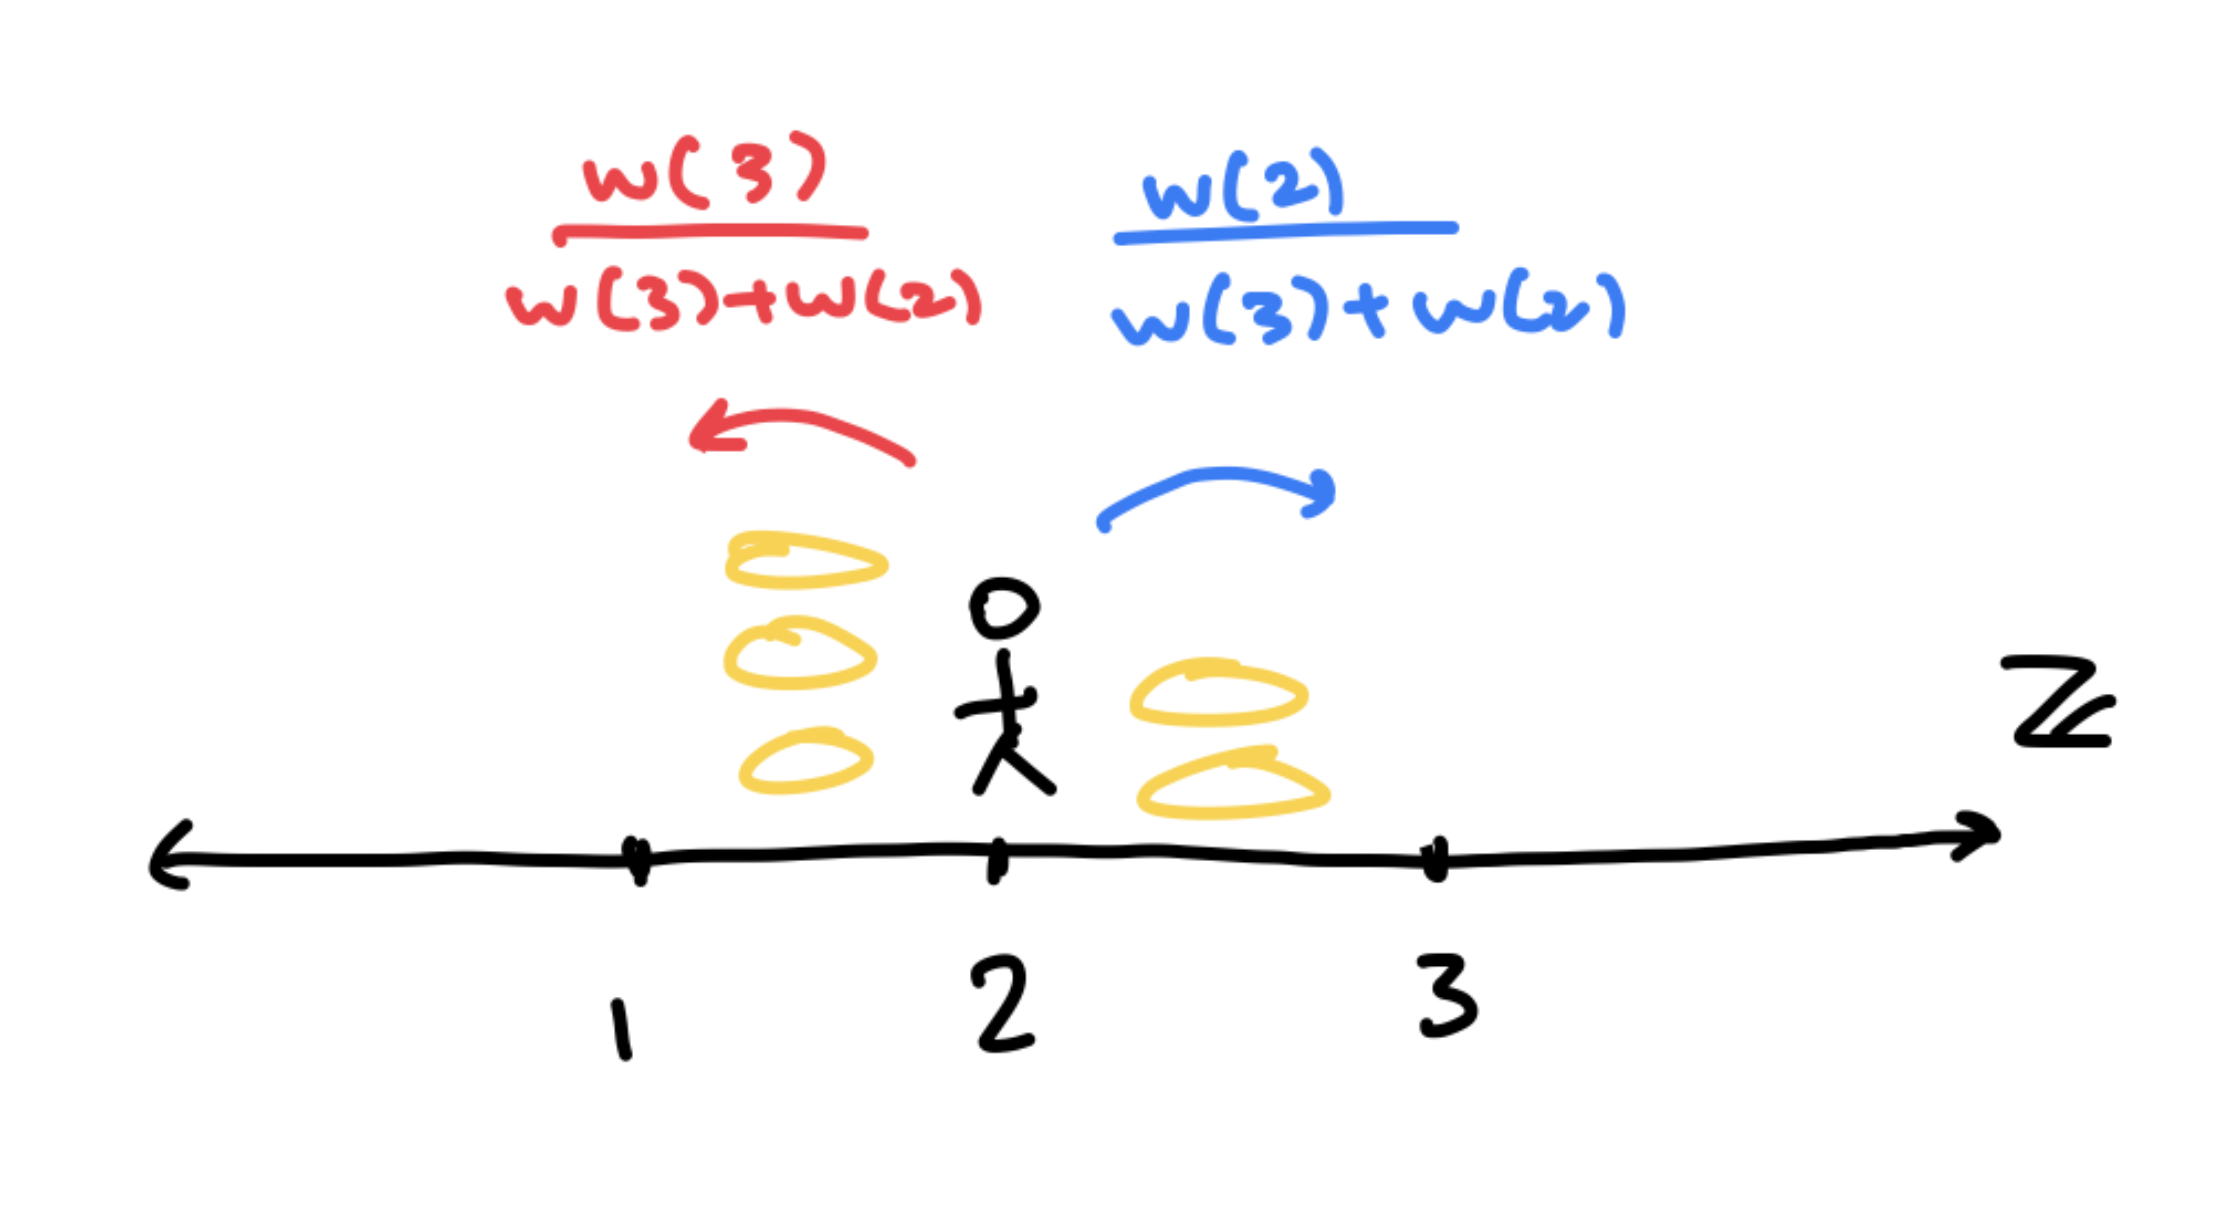
\includegraphics[width=1\linewidth]{src/doodle-def2.png}
    \columnbreak
    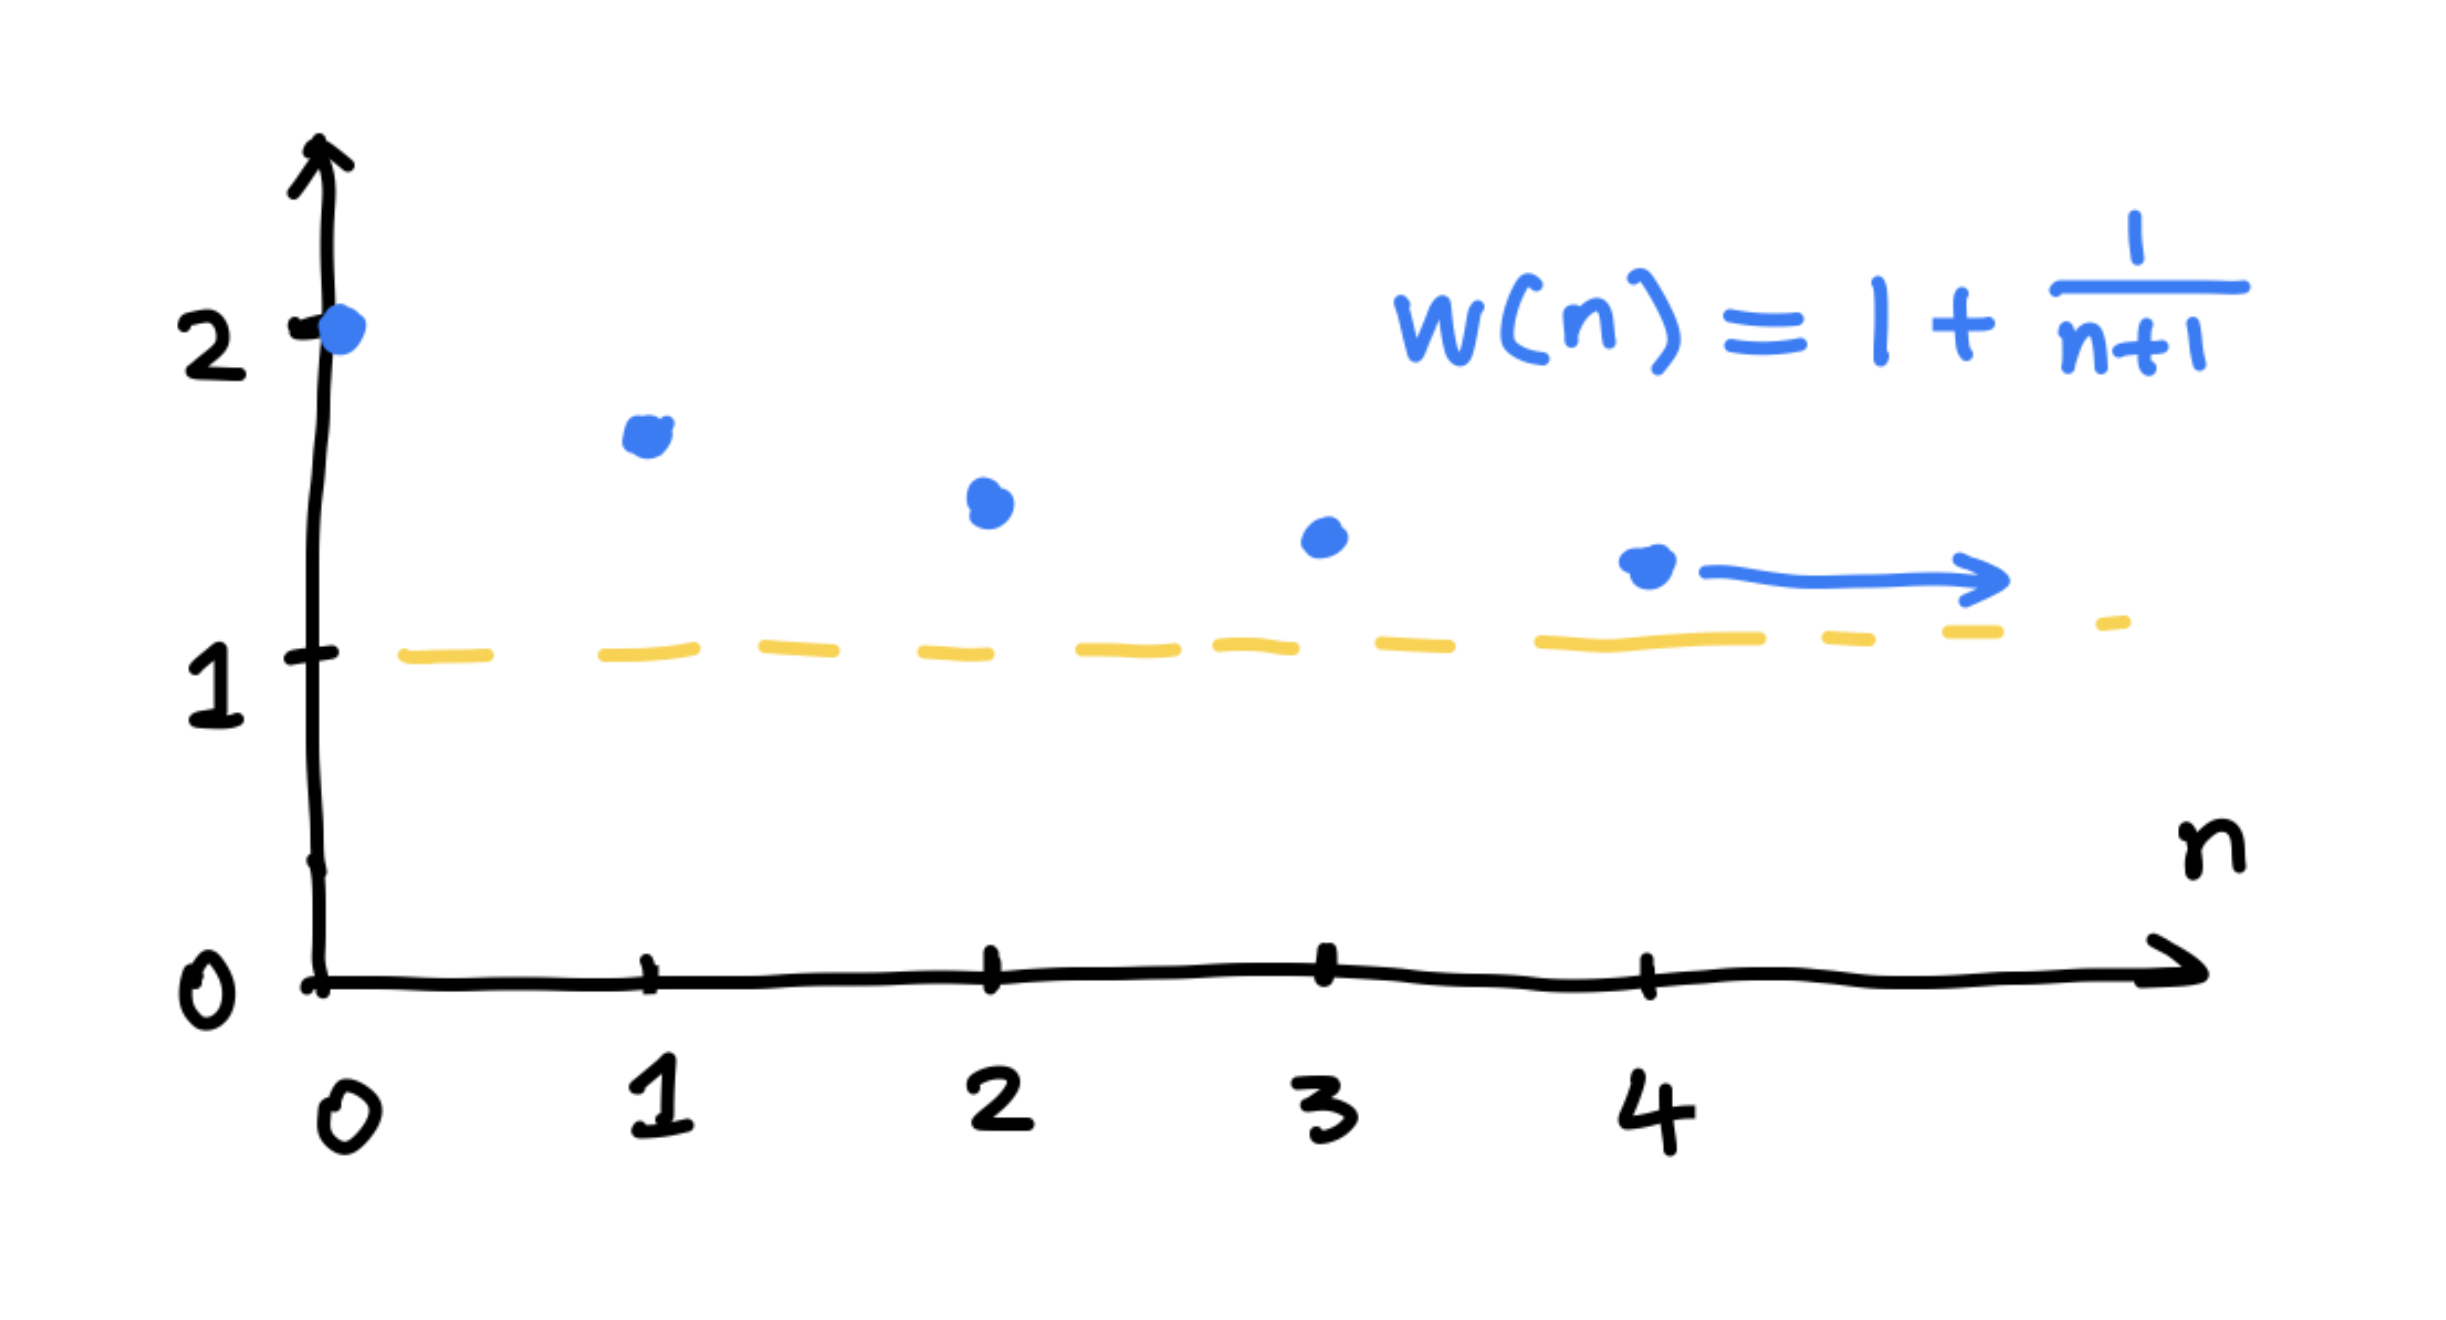
\includegraphics[width=1\linewidth]{src/doodle-def3.png}
    \end{multicols}

    {\color[RGB]{234, 51, 35} How do the SIRWs behave in different parameter regimes? When do we have a functional central limit theorem? }
    We have the following characterization:

    \begin{multicols}{2}
    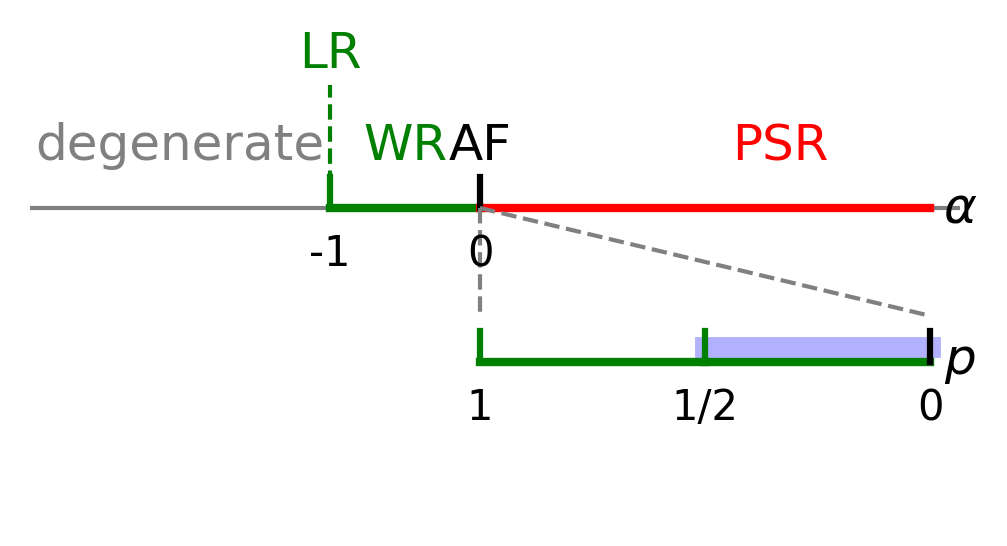
\includegraphics[width=\linewidth]{figures/cases.png}
    \columnbreak

    \textsc{degenerate}: collapse locally [2]\\
    \textsc{Linearly Reinforced}: limiting distribution with no scaling [3]\\
    \textsc{Weakly Reinforced}: limiting distribution with scaling [4]\\
    \textsc{Polynomially Self-repelling}: limiting distribution DNE, one-point distribution open [1] [5]\\
    \textsc{Asymptotically Free}: limiting distribution is BMPE. ([1] identifies the limit, [5] proves $p \in (\frac{1}{2}, 1]$, \thiswork proves $\in (0, \frac{1}{2}]$)
        
    \end{multicols}

    This work completes the picture for the scaling limit of the SIRW in the \textsc{Asymptotically Free} case.
    We show that the phase transition between convergence and non-convergence does not happen for $p \in (0,1)$.

\end{mainbox}

\begin{mainbox}{The walk and the limit}
    The Brownian Motion Perturbed at Extrema (BMPE) is defined as the unique solution of
    \[
    W_t^{\theta^{+}, \theta^{-}}=B_t+\theta^{+} \sup _{s \leq t} W_s+\theta^{-} \inf _{s \leq t} W_s, \quad t \geq 0, \quad W_0=0, \quad \theta^{\pm} < 1,
    \]
    where $B_t$ is a standard Brownian motion [6] [7]. 
    It has a \textit{martingale part} and a \textit{drift part}. A classical technique is to consider the Doob decomposition of the walk
    \[
    X_k = M_k + \Gamma_k
    \]
    which, as we expect, converges to $B_t$ and $\theta^{+} \sup _{s \leq t} W_s+\theta^{-} \inf _{s \leq t} W_s$ respectively.

    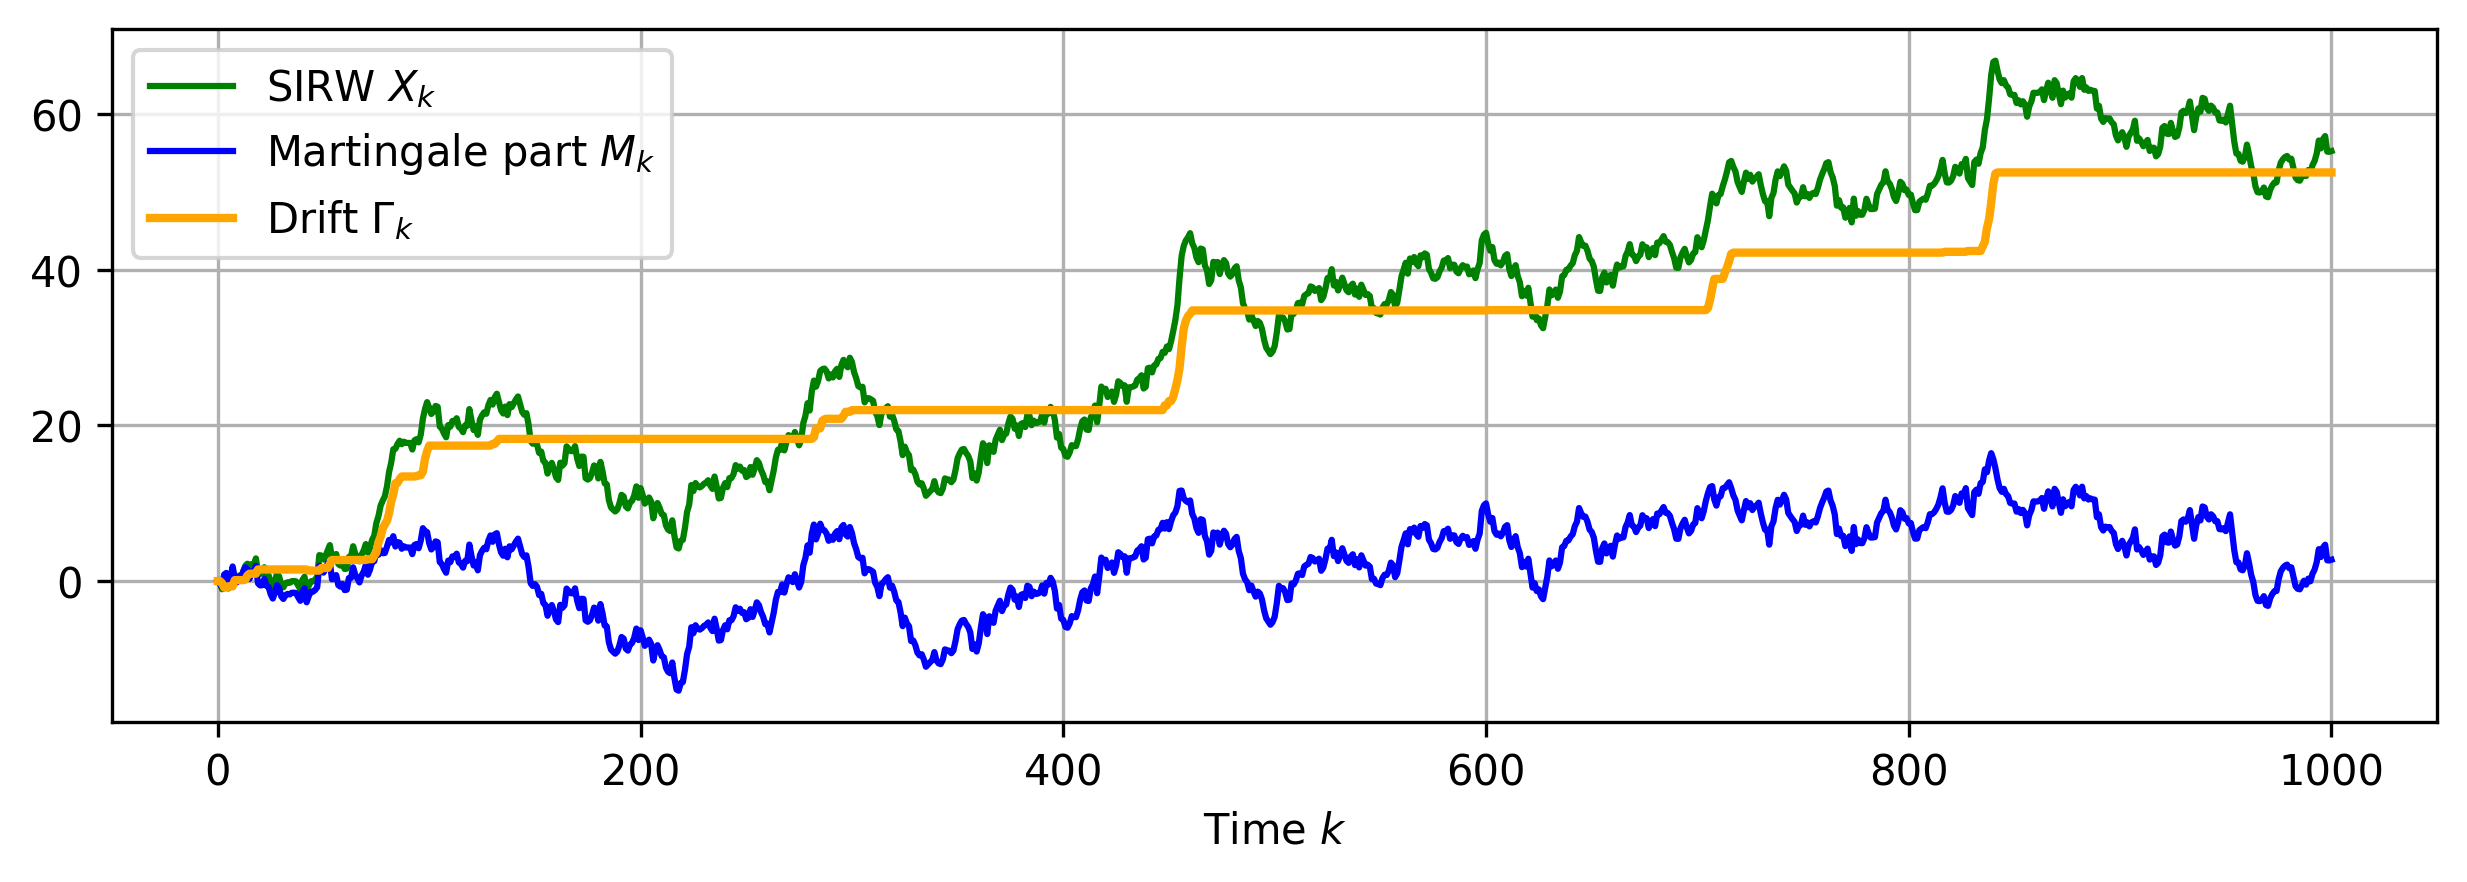
\includegraphics[width=\textwidth]{figures/bmpesmall.png}
\end{mainbox}

\begin{mainbox}{Main Theorem}
Let $w(\cdot)$ be as assumed. For $p \in\left(0, \frac{1}{2}\right]$, and $\kappa>0$. Consider the SIRW $\left(X_k\right)_{k \geq 0}$  with $X_0=0$. We have the following process-level convergence [11]:

\[
\left(\frac{X_{\lfloor n t\rfloor}}{\sqrt{n}}\right)_{t \geq 0} \Longrightarrow\left(W_t^{\gamma, \gamma}\right)_{t \geq 0}
\]

as $n$ goes to infinity, in the standard Skorohod topology on $D([0, \infty))$.

Where, the parameter $\gamma$ is given by
\[
\gamma:=\lim _{m \rightarrow \infty}\left(\sum_{j=0}^{m-1} \frac{1}{w(2 j+1)}-\sum_{j=0}^{m-1} \frac{1}{w(2 j)}\right).
\]
    
\end{mainbox}


\columnbreak

\begin{mainbox}{The generalized Ray-Knight framework}
    The Generalized Ray-Knight Theory [1] states that local time processes of BMPEs $W^{\gamma, \gamma}$ are squared Bessel processes of appropriate dimensions. 
    In the one-dimensional discrete setting, the local time processes of $X_k$ can be explicitly constructed, and their convergence to BESQ processes are established in [1].

    To show process-level convergence of $X_{nt} / \sqrt{n}$ to $W^{\gamma, \gamma}_t$, we follow the following general steps, which have been used in both SIRWs [5] and excited random walks [8] [9] [10].
    
    \begin{itemize}
        \item (Step 1) Convergence of the martingale process $\left( \frac{M_{\left\lfloor n t \right\rfloor}}{\sqrt{n}} \right) _{t \ge 0}$ to $B_t$.
        \item (Step 2) Compare the drift process $\Gamma_k$ to $\gamma (S_k + I_k)$, where $S_k$ and $I_k$ are running maximum and minimum processes of $X_t$.
        \item (Step 3) Process-level tightness of $S_k$ and $I_k$, proved essentially using diffusion approximation.
        \item (Step 4) Conclude convergence of the process triple $\frac{1}{\sqrt{n}}\left(X_{\lfloor n t\rfloor}, M_{\lfloor n t\rfloor}, \Gamma_{\lfloor n t\rfloor}\right)_{t \geq 0}$. %to $\left(Y_1(t), Y_2(t), Y_3(t)\right)_{t \geq 0}$ such that $Y_2$ is standard Brownian motion, $Y_1 = Y_2 + Y_3$, and $Y_3(t)=$ $\gamma\left(\sup _{s \leq t} Y_1(s)+\inf _{s \leq t} Y_1(s)\right)$ for all $t \geq 0, \mathbb{P}$-a.s.
    \end{itemize}
    This approach is used in previous works on one-dimensional excited random walks, and models with site-dependent perturbations.
    One limitation of this approach is the difficulty to generalize to higher dimensions.
\end{mainbox}

\begin{mainbox}{Branching-Like Process}

\begin{multicols}{2}
    Fix a time $k$ where the site local time at $X_k = x$ is $m$. We define the \textit{Branching-Like Process} (BLP) $\left( \zeta^{(x,m)}_k \right) _{k \ge 0}$ as the directed edge local times
    \[
\left(\mathcal{E}_{x+k,+}^{(x, m)}\right)_{k \geq 0}, \quad\left(\mathcal{E}_{x-k,-}^{(x, m)}\right)_{k \geq 0}
\]
as directed edge local times on the event $\{X_k = x, L(x,k) = m\}$. They are Markov processes with respect to spatial filtration.

 Besides, we have the \textit{generalized P\'olya's Urn Process} describes left and right excursions from a single site.
 
%  , with blue balls representing left excursions, and red balls representing right excursions. As a consequence of recurrence, each color is drawn from the urn infinitely often.
\vfill

    \columnbreak
    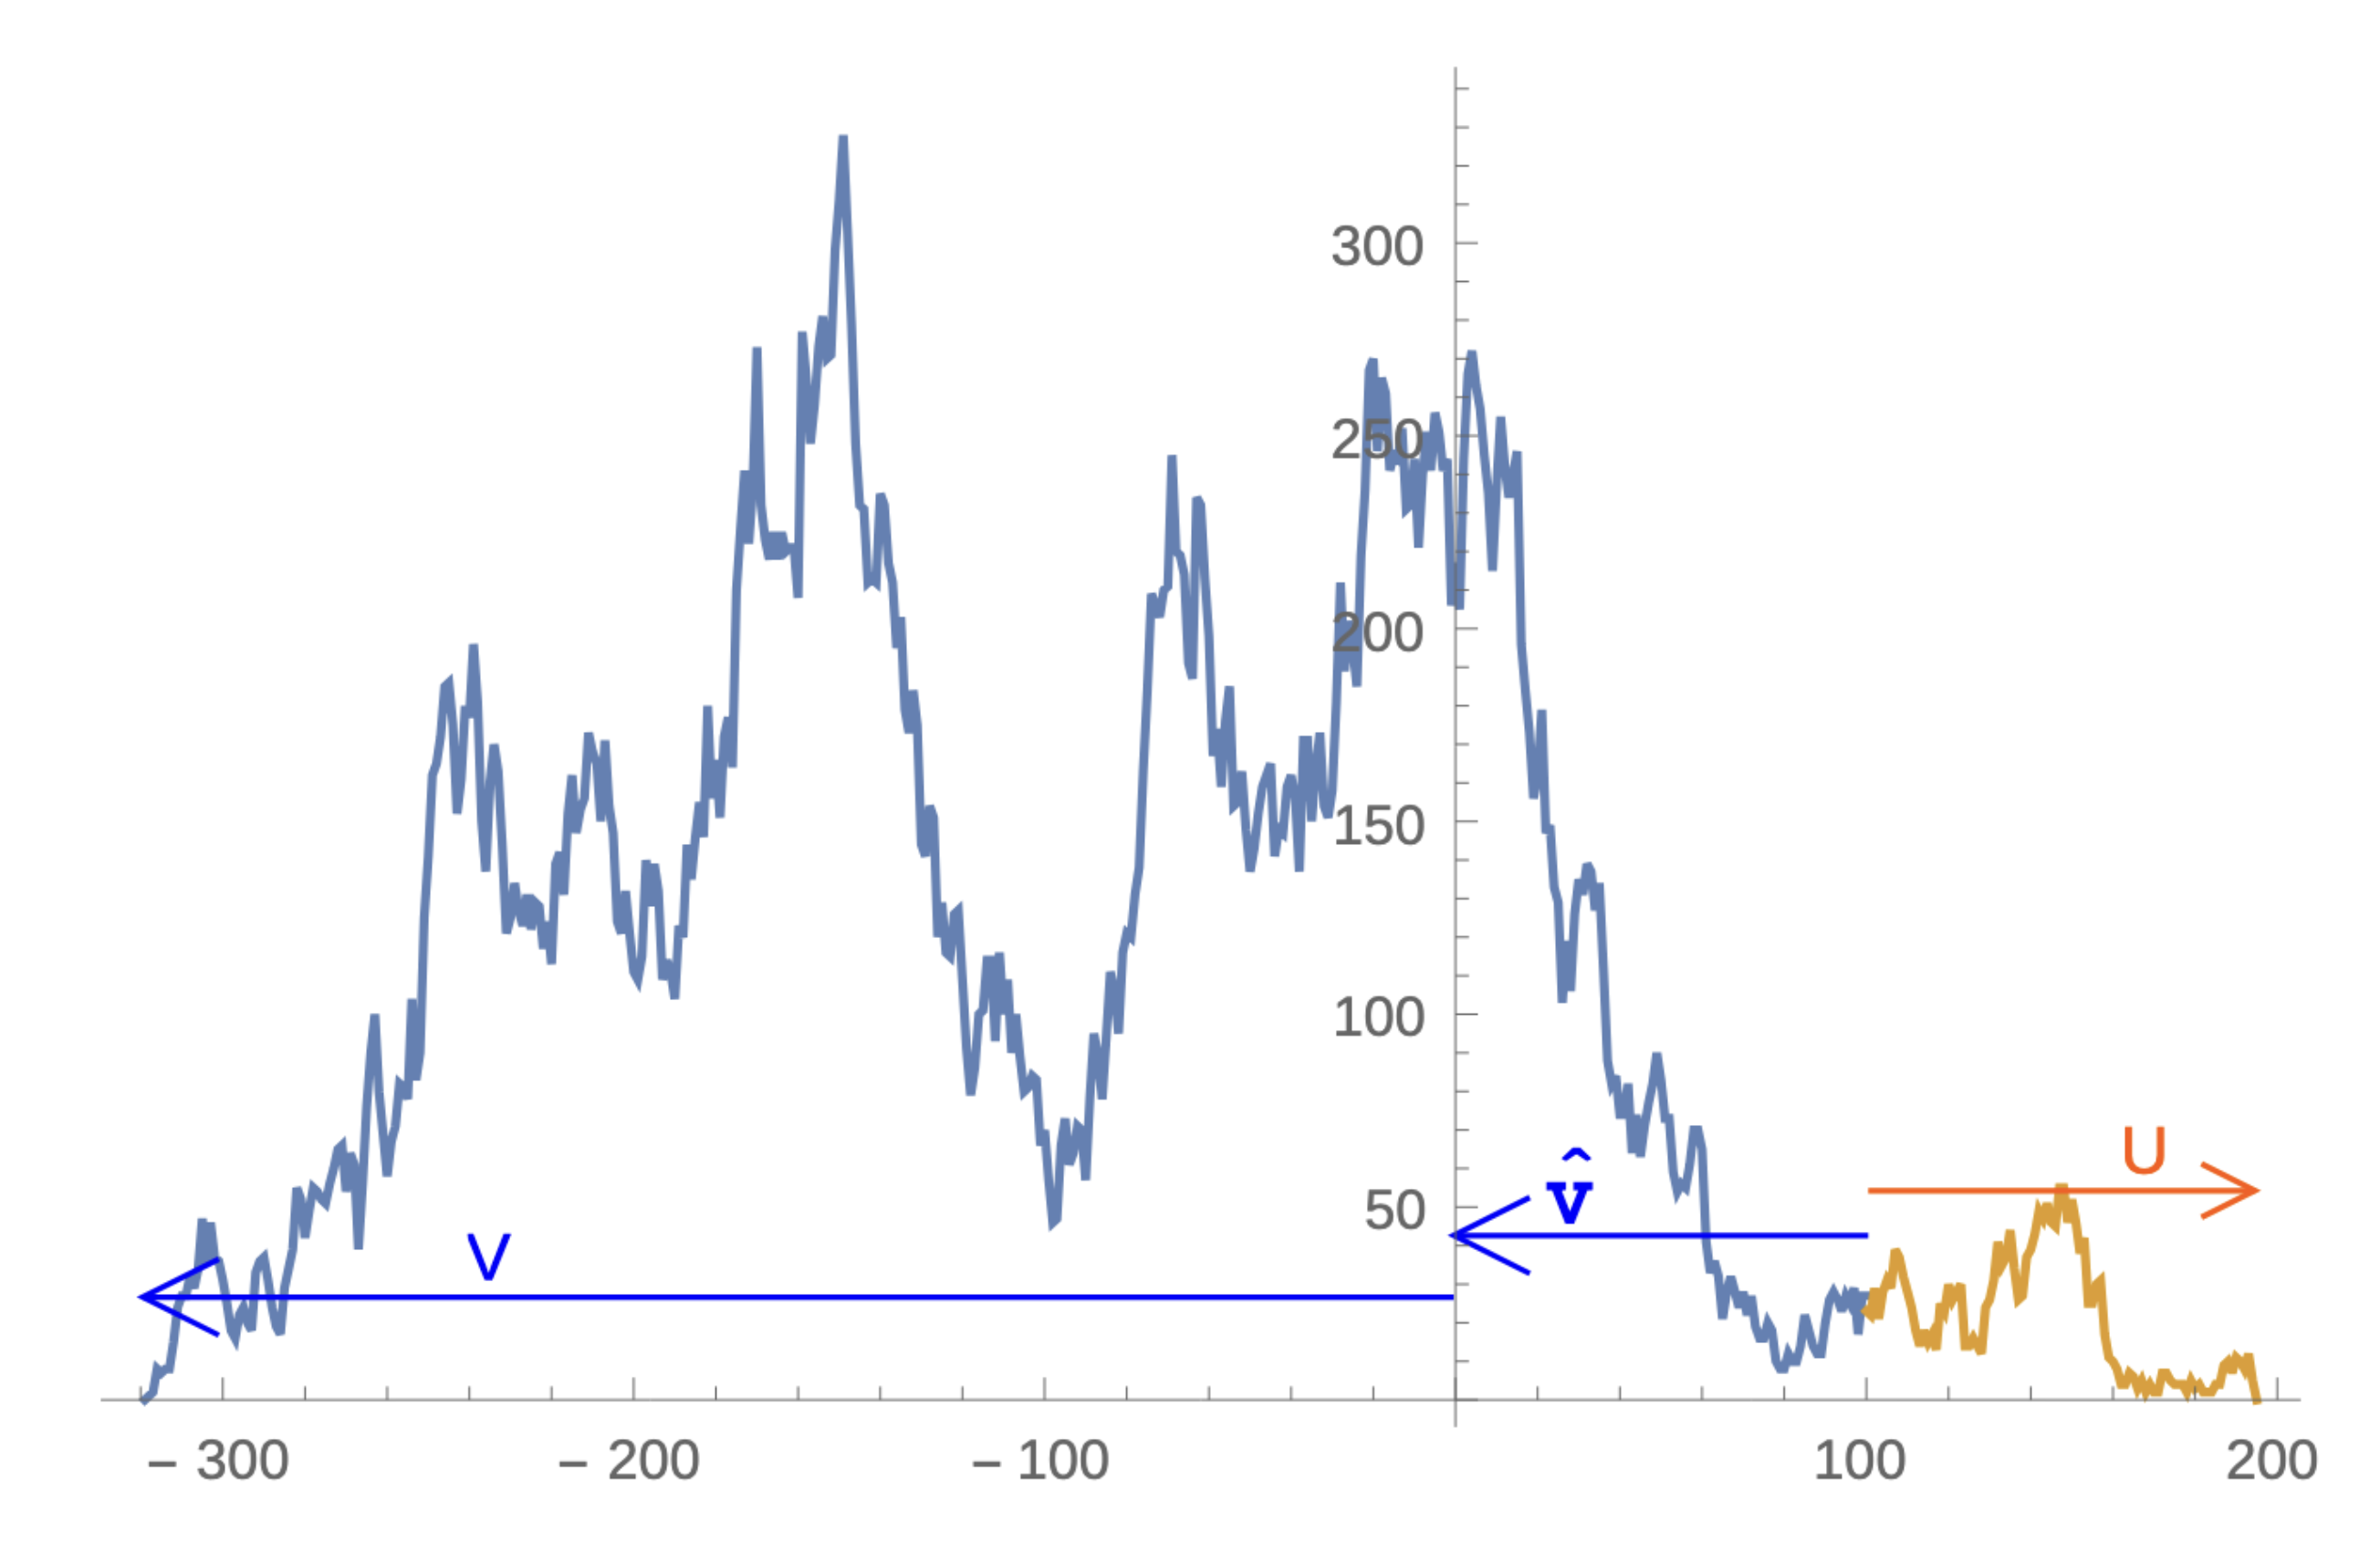
\includegraphics[width=0.8\linewidth]{src/pet16.png}

    Figure: Two types of BLPs [9].

    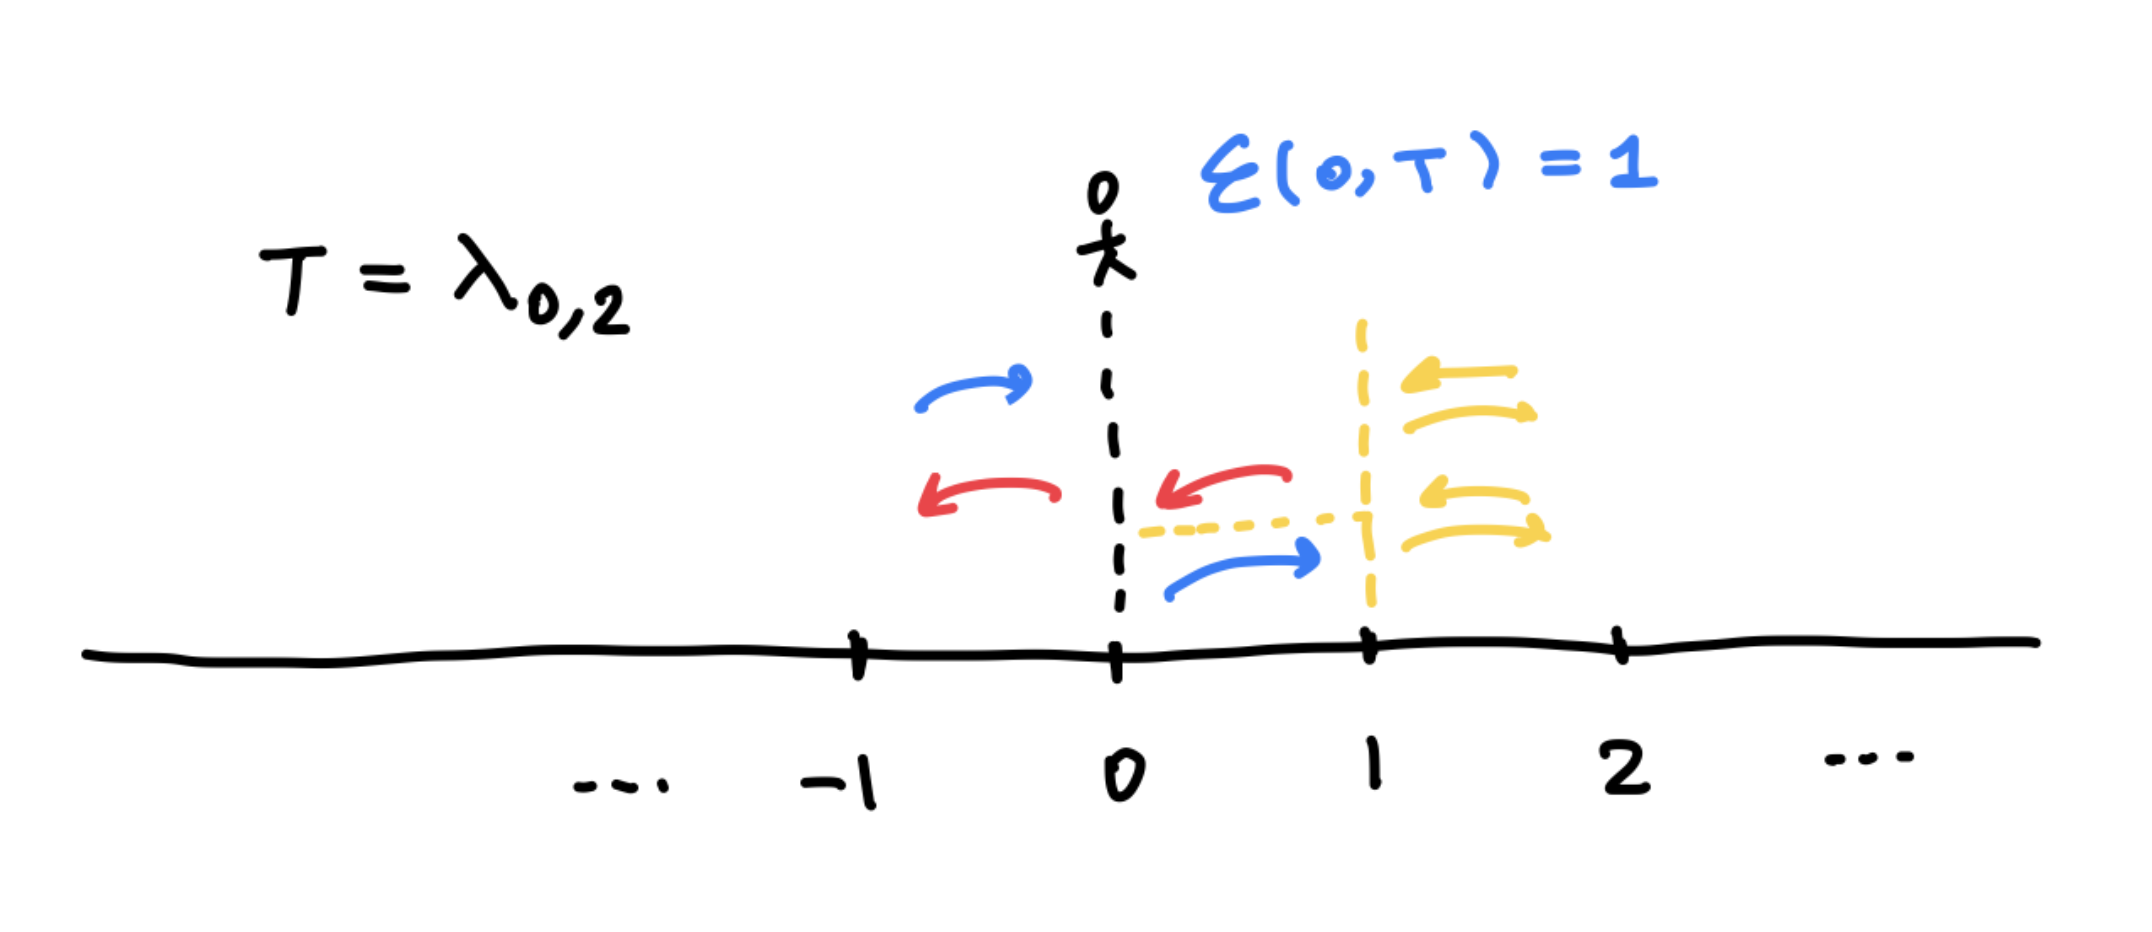
\includegraphics[width=\linewidth]{src/doodle-blp2.png}

    Figure: The directed edge local times.
\end{multicols}

\vspace{0.5in} 

% \begin{multicols}{2}


%     \columnbreak


% \end{multicols}



    
\end{mainbox}

\begin{mainbox}{Diffusion Approximation}
\begin{multicols}{2}
    
\includegraphics[width=0.8\linewidth]{figures/sirwlocal.png}

    \columnbreak
    
\includegraphics[width=0.8\linewidth]{figures/sirwlocalrescaled.png}
\end{multicols}
\begin{center}
    Figure: Local time process of the SIRW, and its limit under diffusive scaling.
\end{center}

    In the lemma below, let $\sigma_0^Z$ be the first hitting time of level $0$ for a process $\left( Z_t \right) _{t \in [0,\infty )}$ starting from a positive value, i.e. $\sigma_0^Z := \inf \{t>0: Z_t \le 0\} $.
(Proposition A.3 [5]]; Theorem 1A [1])
	\begin{enumerate}
		\item 
		For $n\geq 1$, let $\zeta^{(n)}=(\zeta^{(n)}_k)_{k\geq 0 }  $ be the first type BLP with initial value $\zeta^{(n)}_0 = \lfloor yn \rfloor$ for some $y \geq 0$, and let $\mathcal{Z}_n(t) = \frac{\zeta^{(n)}_{\lfloor nt \rfloor}}{n}$ for $n\geq 1$ and $t\geq 0$. Then we have that 
		\[
		\mathcal{Z}_n(.) \Longrightarrow Z^{(2-2\gamma)}(.)
		\] 
		as $n$ goes to infinity on $D([0,\infty))$, where $2Z^{(2-2\gamma)}(.)$ is a squared Bessel process of dimension $2-2\gamma$, with $Z^{(2 - 2 \gamma)}(0) = y$.
		
		\item
		For the second type BLP, we have that 
		\[
		\left(\tilde{\mathcal{Z}}_n(.), \sigma_0^{\tilde{\mathcal{Z}}_n}\right) 
		\Longrightarrow \left(Z^{(2\gamma)}(. \wedge \sigma_0^{Z^{(2 \gamma)}}), \sigma_0^{Z^{(2 \gamma)}}\right).
		\]
	\end{enumerate}
	
	

\end{mainbox}

\columnbreak
% \begin{mainbox}{Good Events}
%     \begin{multicols}{2}
%     \begin{align}
%         G_{n,K,t} :=  \qquad
%         \label{eq:good-event-1}
%         & \left\{\sup _{k \le \left\lfloor nt  \right\rfloor} |X_k| < K \sqrt{n} \right\} \cap \\
%         \label{eq:good-event-2}
%         & \left\{\sup_{y \in \mathbb{Z}} L(y, \left\lfloor nt  \right\rfloor) < K \sqrt{n} \right\} \cap \\
%         \label{eq:good-event-3}
%         & \bigcap_{y = - K \sqrt{n} }^{K \sqrt{n}} 
%         \bigcap_{i = 1}^{K \sqrt{n} } \left\{\left| \tau_{i,y}^{\mathscr{B}} - 2 i \right| < \sqrt{ i } \log^2 n \right\}  \cap \\
%         \label{eq:good-event-4}
%         & \bigcap_{y = - K \sqrt{n} }^{K \sqrt{n}} 
%         \bigcap_{i = 0}^{K \sqrt{n} } \left\{\left| \tau_{i+1, y}^{\mathscr{B}} - \tau_{i,y}^{\mathscr{B}} \right| < \log^2 n \right\}  
%         .\end{align}
%    \columnbreak
%     \begin{align}
%         G_{n,K}^{(x,m)}(y) :=  \qquad
%         \label{eq:good-event-5}
%         & \left\{L(y,\lambda_{x,m})  < K \sqrt{n} \right\} \cap \\
%         \label{eq:good-event-6}
%         & \left\{\left| \tau_{i,y}^{\mathscr{B}} - 2 i \right| < \sqrt{ i } \log^2 n, \mbox{for all $i\leq  \mathcal{E}_{y,-}^{(x,m)}$} \right\}  \cap \\
%         \label{eq:good-event-7}
%         & \left\{\left| \tau_{i+1,y}^{\mathscr{B}} - \tau_i^{\mathscr{B},y} \right| < \log^2 n,  \mbox{for all $i\leq  \mathcal{E}_{y,-}^{(x,m)}$}  \right\}  
%         .\end{align}
%     \end{multicols}
% \end{mainbox}
\begin{mainbox}{Good Events, Two-step Approximation}
    \begin{multicols}{2}
    [To complete steps (1), (2) and (3), we work on good events $G_{n,K,t}$ and its ``procedual realization'' $G_{n,K}^{(x,m)}(y)$ adapted to the BLP filtration. Those events are proved typical via concentration-type inequalities associated to the BLP and the P\'olya's urn process (excursions).]
    \vspace{-1em}
    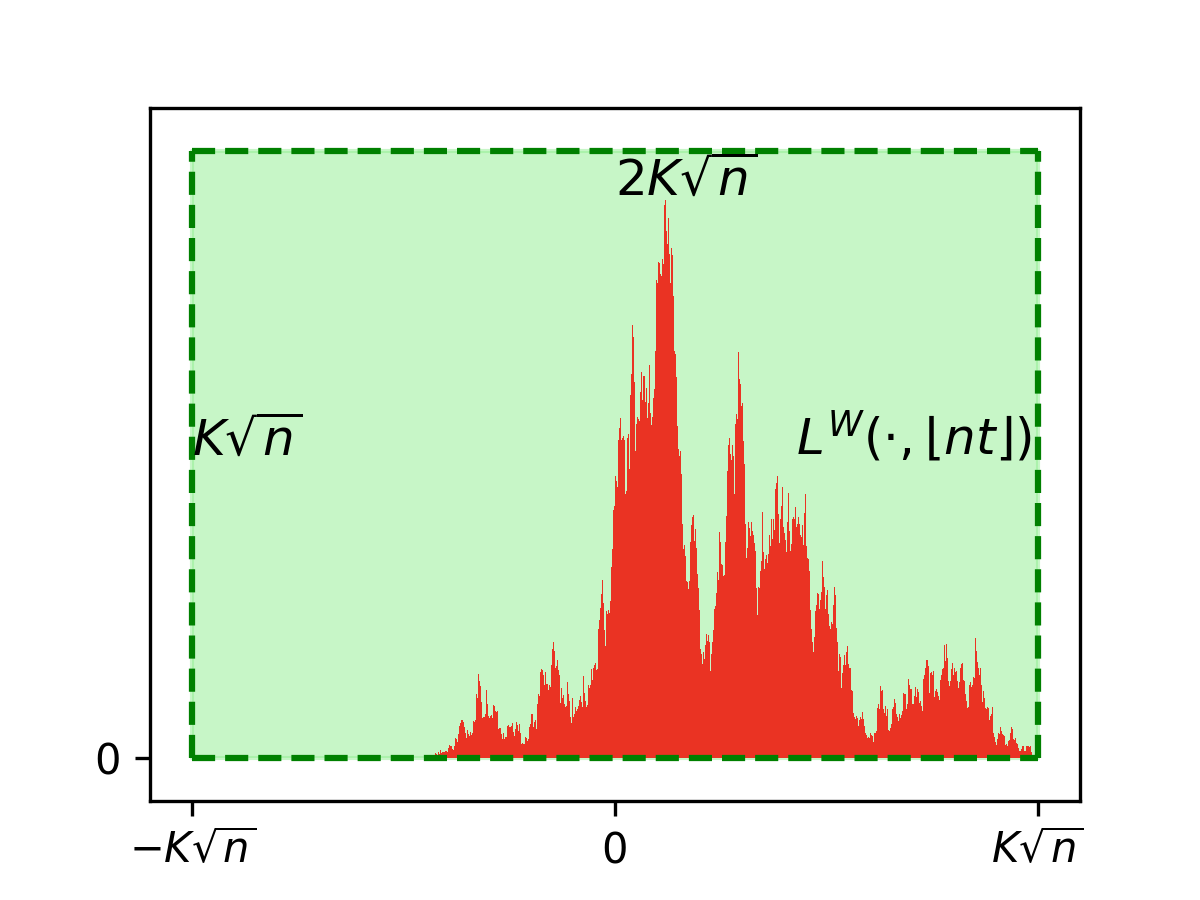
\includegraphics[width=0.8\linewidth]{figures/goodevent.png}

    \columnbreak
    Figure: The good event $G_{n,K,t}$ is defined such that three things happen up to time $\lfloor nt \rfloor$: \\
    (1) Range of walk is bounded by $K \sqrt{n}$ from up and below,\\ (2) Local time at each site is bounded by $K \sqrt{n}$, \\
    (3) The P\'olya's urn processes are well-behaved inside the controlled region, with approximately same numbers of red and blue balls drawn. 
    \end{multicols}
% \begin{figure}[htbp]
%     \centering
%     \begin{minipage}[t]{0.48\textwidth}
%       \centering
%       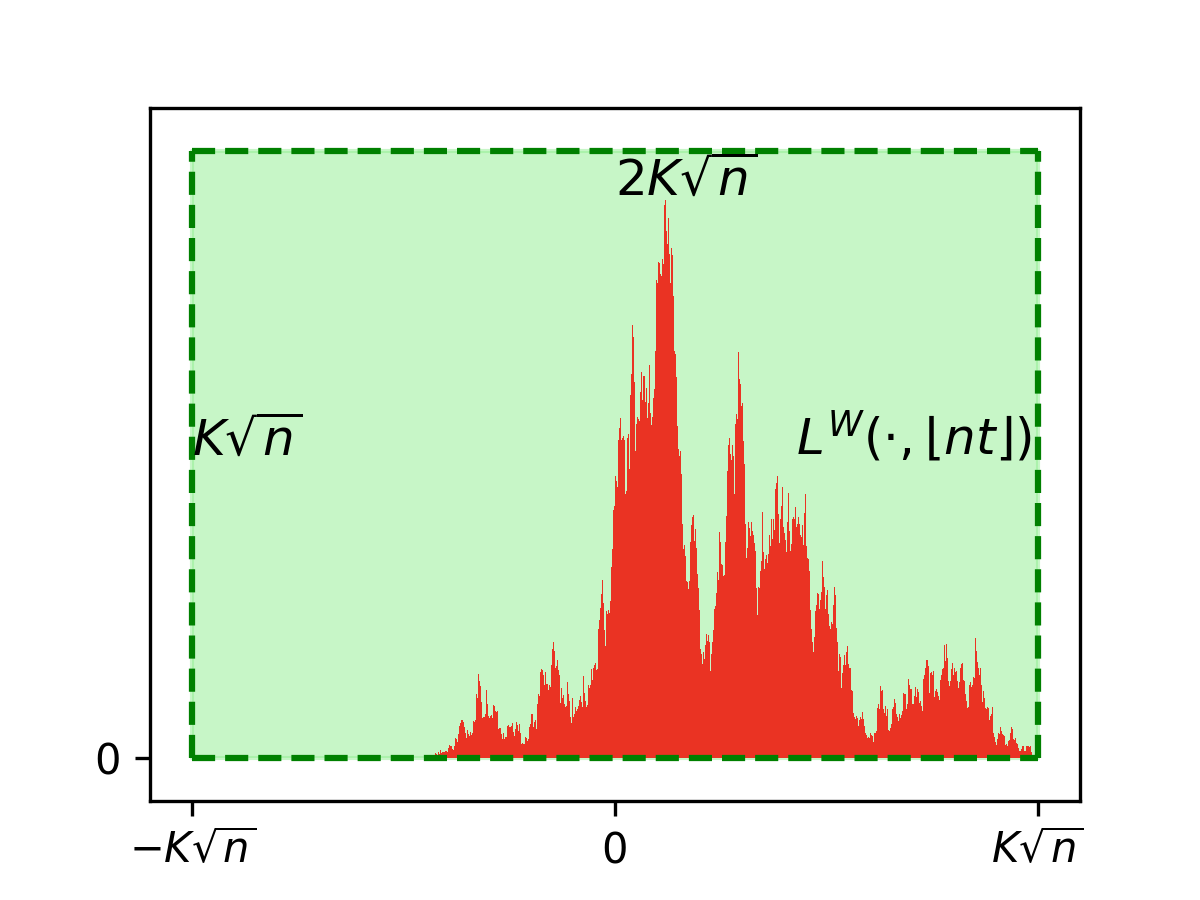
\includegraphics[width=\linewidth]{figures/goodevent.png}
%     \end{minipage}
%     % \hfill
%     \begin{minipage}[t]{0.48\textwidth}
%       \small % or \footnotesize for compactness
%       \textbf{Figure:} The good event $G_{n,K,t}$ is defined such that three things happen up to time $\lfloor nt \rfloor$: (1) Range of walk is bounded by $K\sqrt{n}$, (2) Local time at each site is bounded by $K\sqrt{n}$, (3) The Pólya’s urn processes are well-behaved in this region.
%     \end{minipage}
%   \end{figure}
% \end{mainbox}
% \begin{mainbox}{Two-step Approximation}
    Let $\rho_y^{(x, m)}=\mathbb{E}\left[\Delta_y^{(x, m)} \mid \mathcal{G}_{y-1}^{(x, m)}\right]$. 
    $\mathcal{G}_{y-1}^{(x, m)}$ is the filtration generated by the BLP. This gives a spatial martingale describing the drift.
    Convergence of $\Gamma_k$ follows from
    \[
\lim _{n \rightarrow \infty} \mathbb{P}\left(\sup _{k \leq\lfloor n t\rfloor}\left|\sum_{y>X_k}\left(\rho_y^{\left(X_k, L\left(X_k, k\right)-1\right)}-\gamma \cdot \operatorname{sgn}(y)\right)\right|>\varepsilon \sqrt{n}\right)=0 .
\]
and
\[
\lim _{n \rightarrow \infty} \mathbb{P}\left(\sup _{k \leq\lfloor n t\rfloor}\left|\sum_{y>X_k}\left(\Delta_y^{\left(X_k, L\left(X_k, k\right)-1\right)}-\rho_y^{\left(X_k, L\left(X_k, k\right)-1\right)}\right)\right|>\varepsilon \sqrt{n}\right)=0 .
\]
The first one is analyzed using Polya's urn process on the good event.
The second one is controlled on the good event where the drift forms a spatial martingale with bounded increments.

\end{mainbox}
\begin{mainbox}{Future Directions}
    \begin{itemize}
        \item Relax assumptions on weight function, e.g. consider non-monotone weight function.
        \item Convergence of one-dimensional distributions of the \textsc{Polynomially Self-Repelling} SIRW to BMPE is to be studied.
    \end{itemize}
\end{mainbox}

\begin{mainbox}{Acknowledgements}
    Xiaoyu Liu gratefully acknowledges the support from the Purdue Mathematics Department through the Joel Spira Research Fellowship (2023). Zhe Wang gratefully acknowledges the support from the Swiss National Science Foundation, grant 200021L -- 169691. Both authors thank \textbf{Prof. Jonathon Peterson} and \textbf{Prof. Thomas Mountford} for their suggestion of the problem and for enriching discussions.
\end{mainbox}
\begin{mainbox}{References}
    \begingroup
\renewcommand{\section}[2]{}%
    \providecommand{\bysame}{\leavevmode\hbox to3em{\hrulefill}\thinspace}
\providecommand{\MR}{\relax\ifhmode\unskip\space\fi MR }
% \MRhref is called by the amsart/book/proc definition of \MR.
\providecommand{\MRhref}[2]{%
  \href{http://www.ams.org/mathscinet-getitem?mr=#1}{#2}
}
\providecommand{\href}[2]{#2}
\begin{thebibliography}{10}
        
        \bibitem{T96}
        T\'{o}th,~B.: Generalized {R}ay-{K}night theory and limit theorems for self-interacting random walks on {${\bf Z}^1$}, \emph{Ann. Probab.} \textbf{24} (1996), no.~3, 1324--1367. \MR{1411497}
        
        \bibitem{Dav96}
        Davis,~B.: Weak limits of perturbed random walks and the equation {$Y_t=B_t+\alpha\sup\{Y_s\colon\ s\leq t\}+\beta\inf\{Y_s\colon\ s\leq t\}$}, \emph{Ann. Probab.} \textbf{24} (1996), no.~4, 2007--2023. \MR{1415238}
        




        \bibitem{P88}
        Pemantle,~R.: Phase transition in reinforced random walk and {RWRE} on trees, \emph{Ann. Probab.} \textbf{16} (1988), no.~3, 1229--1242. 

        \bibitem{T97}
        T\'{o}th,~B.: Limit theorems for weakly reinforced random walks on {Z}, \emph{Studia Scientiarum Mathematicarum Hungarica} \textbf{33} (1997), no.~1--3, 321--337.

        \bibitem{KMP23}
        \bysame, Convergence and nonconvergence of scaled self-interacting random walks to {B}rownian motion perturbed at extrema, \emph{Ann. Probab.} \textbf{51} (2023), no.~5, 1684--1728. \MR{4642221}

        \bibitem{CPY98}
        Carmona,~P., Petit,~F., Yor,~M.: Beta Variables as Times Spent in [0, $\infty$[ By Certain Perturbed Brownian Motions, \emph{Journal of the London Mathematical Society} \textbf{58} (1998), no.~1, 239--256.

        \bibitem{Dav99}
        \bysame, Brownian motion and random walk perturbed at extrema, \emph{Probab. Theory Related Fields} \textbf{113} (1999), no.~4, 501--518. \MR{1717528}

        
        \bibitem{DK12}
        Dolgopyat,~D., Kosygina, E.: Scaling limits of recurrent excited random walks on integers, \emph{Electron. Commun. Probab.} \textbf{17} (2012), no. 35, 14. \MR{2965748}

        
        \bibitem{KP16}
        Kosygina,~E., Peterson,~J.: Functional limit laws for recurrent excited random walks with periodic cookie stacks, \emph{Electron. J. Probab.} \textbf{21} (2016), Paper No. 70, 24. \MR{3580036}

                
        \bibitem{KMP22}
        Kosygina,~E., Mountford,~T., Peterson,~J.: Convergence of random walks with {M}arkovian cookie stacks to {B}rownian motion perturbed at extrema, \emph{Probab. Theory Related Fields} \textbf{182} (2022), no.~1-2, 189--275. \MR{4367948}
        


        
      
        \bibitem{B99}
        Billingsley,~P.: \emph{Convergence of probability measures} (1999).
        


        
        \end{thebibliography}
        \endgroup
    % 1 T96 \\
    % 2 Davis 1990\\
    % 3 Pemantle 1988 \\
    % 4 T96 (WR) \\
    % 5 BMP23 \\
    % 6 Carmona, Petit and Yor (1995) and \\
    % 7 Davis (1995)\\
    % 8 Dolgopyat 12\\
    % 9 KP16 \\
    % 10 KMP22 \\
\end{mainbox}